\chapter{The Prototyping Mindset \& the Workflow}
\label{ch2}

Every prototype you build costs time, materials, and opportunity.
Build the wrong one --- too early, too polished, or targeting the wrong
question --- and you burn weeks that a one-day breadboard experiment would
have saved.
This chapter gives you the reasoning scaffold that prevents that waste: the
\textbf{Prototype Development Cycle}\index{Prototype Development Cycle}, a
seven-stage process that turns an ambiguous project brief into a disciplined
sequence of validated decisions.
By the end of the chapter you will be able to plan a prototype, defend your
fidelity choice with arithmetic, and hand a concise question statement to
any reviewer, client, or collaborator.

\bigskip
\noindent\textbf{Learning Objectives.}
After working through this chapter you will be able to:
\begin{enumerate}
  \item Walk through all seven stages of the Prototype Development Cycle and
        explain the purpose of each.
  \item Define a prototype by the question it answers and the risk it reduces.
  \item Apply the controlled Design\,$\leftrightarrow$\,Validate iteration
        loop correctly.
  \item Select the appropriate prototype type for a given engineering question.
  \item Choose fidelity deliberately based on the question, not habit.
\end{enumerate}

%%%%%%%%%%%%%%%%%%%%%%%%%%%%%%%%%%%%%%%%%%%%%%%%%%%%%%%%%%%%%%%%%%%%%%%%%%%
\section{Prototype = Answer to a Question, Reducer of Risk}
\label{sec:ch2-question}
%%%%%%%%%%%%%%%%%%%%%%%%%%%%%%%%%%%%%%%%%%%%%%%%%%%%%%%%%%%%%%%%%%%%%%%%%%%

A prototype is not a small version of the final product.
It is not a demonstration for a trade show, a proof that your team is
making progress, or practice for the real build.
A prototype is a \textbf{minimum sufficient artifact}\index{prototype!definition}
constructed to answer one specific technical or business question and to
retire a corresponding risk.

Write the question down before you pick up a soldering iron.
If you cannot write it in a single sentence, you do not yet know what you
are building.
Consider the difference between these two framings:

\begin{itemize}
  \item \emph{Vague:} ``We need to build a prototype of the sorter.''
  \item \emph{Precise:} ``Can a sub-\$500~CAD BOM sorter module achieve
        $\geq$95\,\% sort accuracy at 6~items/min with reliable MQTT
        connectivity over standard Wi-Fi?''
\end{itemize}

The precise framing tells you exactly what to build (a low-cost sorter
mechanism with Wi-Fi MQTT), what to measure (accuracy at a fixed throughput
rate), and what threshold constitutes a ``yes'' answer.
It also tells you what \emph{not} to build: an injection-moulded housing,
CE-marked power supply, or production PCB layout are irrelevant until the
accuracy and connectivity question is answered.

\textbf{Risk}\index{risk!in prototyping} in this context is the probability
that an unverified assumption collapses the project.
Every assumption you have not tested is a risk.
A prototype converts an assumption into a measurement, and a measurement
into a decision.
Figure~\ref{fig:ch2-value} shows how even a low-fidelity prototype delivers
substantial intrinsic value --- knowledge and risk reduction --- long before
artifact quality approaches production standards.

\begin{figure}[htbp]
  \centering
  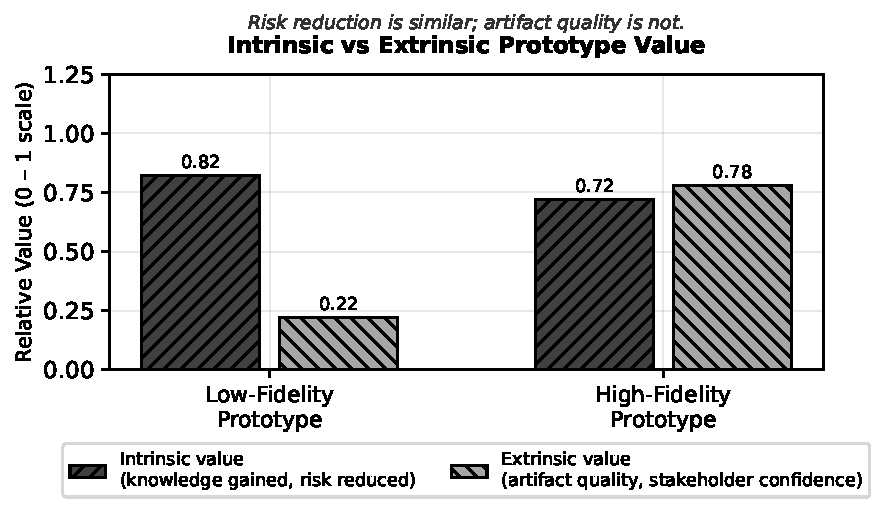
\includegraphics[width=0.85\textwidth]{images/fig_03_value.pdf}
  \caption{Intrinsic value (knowledge, risk reduction) is substantial even at low
           fidelity; extrinsic value (artifact quality, stakeholder confidence)
           grows mainly at high fidelity. Build to the fidelity the question
           requires, not the fidelity that impresses.}
  \label{fig:ch2-value}
\end{figure}

The discipline of framing every build as an answer to a question keeps your
team aligned and prevents the single most common prototyping failure: building
features that are not yet questions.

%%%%%%%%%%%%%%%%%%%%%%%%%%%%%%%%%%%%%%%%%%%%%%%%%%%%%%%%%%%%%%%%%%%%%%%%%%%
\section{The Seven Stages}
\label{sec:ch2-seven-stages}
%%%%%%%%%%%%%%%%%%%%%%%%%%%%%%%%%%%%%%%%%%%%%%%%%%%%%%%%%%%%%%%%%%%%%%%%%%%

Figure~\ref{fig:ch2-workflow} shows the full Prototype Development Cycle.
The seven stages run left to right; Stages~4 through~6 form the core
build-test loop that iterates until the central question is answered.
The loop is controlled --- you exit it on a criterion, not when you run out
of time.

\begin{figure}[htbp]
  \centering
  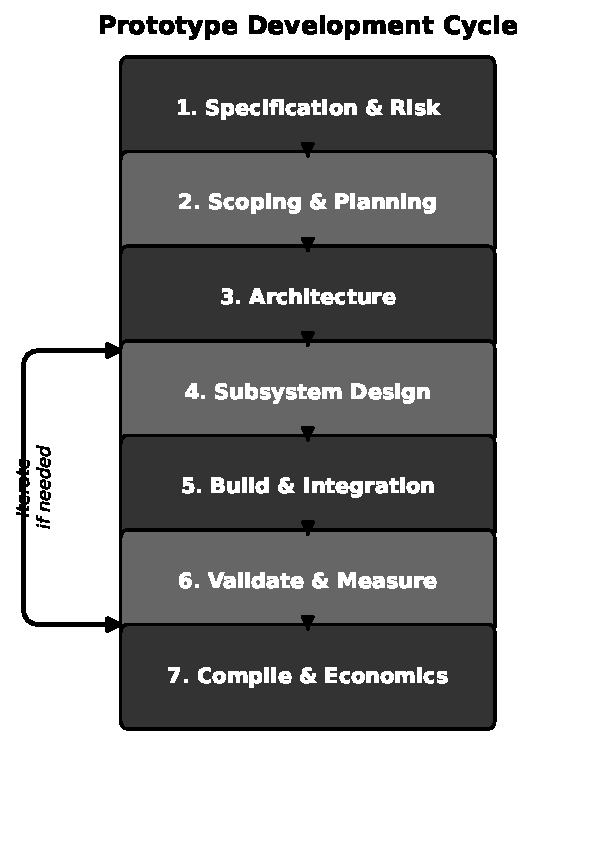
\includegraphics[width=0.85\textwidth]{images/fig_01_workflow.pdf}
  \caption{The seven-stage Prototype Development Cycle with the Design\,$\leftrightarrow$\,Validate
           iteration loop. Stages~4 through~6 form the core build-test loop;
           iteration is controlled, not ad-hoc.}
  \label{fig:ch2-workflow}
\end{figure}

%---------------------------------------------------------------------------
\subsection{Stage~1: Specification \& Risk}
\label{sec:ch2-stage1}
%---------------------------------------------------------------------------

Stage~1 transforms the project brief into a structured set of
\textbf{specifications}\index{specification} and a ranked list of
\textbf{risks}\index{risk!list}.
You are not designing anything yet.
You are reading, asking questions, and writing.

A specification at this stage has four components:
\begin{enumerate}
  \item \emph{Functional requirements} --- what the system must do
        (``sort at $\geq$6~items/min'').
  \item \emph{Performance bounds} --- measurable thresholds
        (``$\geq$95\,\% accuracy'', ``MQTT round-trip $\leq$200\,ms'').
  \item \emph{Constraints} --- non-negotiable limits
        (``BOM cost $\leq$\$500~CAD'', ``fits on a 600\,mm bench conveyor'').
  \item \emph{Assumptions} --- things believed to be true but not yet measured.
\end{enumerate}

Every assumption in item~4 is a risk candidate.
You rank risks by the product of probability and impact, and you identify
which prototype stage will retire each one.
By the end of Stage~1 you have a written specification document and a risk
register.
These are the two artifacts that every subsequent stage references.

\paragraph{In Practice.}
A one-hour specification session with your full team at the whiteboard saves
more time than a week of uncoordinated building.
Force every team member to write at least one assumption.
Assumptions that no one writes down are the ones that kill projects in
Week~10.

%---------------------------------------------------------------------------
\subsection{Stage~2: Scoping \& Planning}
\label{sec:ch2-stage2}
%---------------------------------------------------------------------------

Stage~2 converts the risk register into a prototype plan.
You decide: which risks must be retired by this prototype, what fidelity
level is sufficient to retire them, how long the build will take, and what
success looks like.

The key output is a \textbf{prototype plan}\index{prototype plan} with:
\begin{itemize}
  \item The central question (one sentence).
  \item The chosen fidelity level and justification.
  \item A work-breakdown with task ownership and duration.
  \item Explicit pass/fail criteria for the validation step.
\end{itemize}

Scoping means saying ``not this prototype.''
If the question is about sort accuracy, the housing material is out of scope.
Resist the urge to answer every question at once; you will get a chance in
the next milestone.
A well-scoped prototype plan is a document your supervisor can review in
ten minutes and approve or correct before your team spends any build time.

%---------------------------------------------------------------------------
\subsection{Stage~3: Architecture}
\label{sec:ch2-stage3}
%---------------------------------------------------------------------------

Stage~3 partitions the system into \textbf{subsystems}\index{subsystem} with
defined interfaces.
You are not selecting components yet; you are drawing boundaries.

A useful architecture diagram shows:
\begin{itemize}
  \item Each subsystem as a labelled block.
  \item Every signal and power interface as an arrow with direction and type
        (digital, analog, mechanical, protocol name).
  \item The measurement points where validation data will be collected.
\end{itemize}

The architecture is the contract between team members.
If two people are building adjacent subsystems without an agreed interface,
integration will fail.
In Stage~3 you negotiate and document those contracts before anyone starts
detailed design.

Architecture decisions also constrain which subsystem risks are separable.
If sort accuracy depends on both the sensor subsystem and the conveyor speed
controller, you cannot test one without the other --- and your plan must
reflect that coupling.

%---------------------------------------------------------------------------
\subsection{Stage~4: Subsystem Design}
\label{sec:ch2-stage4}
%---------------------------------------------------------------------------

Stage~4 is detailed design: component selection, schematic capture, firmware
architecture, mechanical part design, and BOM costing.
This is where your prior coursework in PCB design, embedded programming, and
mechanical CAD becomes the primary activity.

In a prototype context, Stage~4 output does not need to be production-ready.
A breadboard schematic is a legitimate Stage~4 artifact if it enables the
Stage~5 build to proceed and the Stage~6 measurement to be valid.
Keep every design decision traceable to a specification line or a risk item.
If you cannot trace it, question whether you need it.

Stage~4 is the entry point to the Design\,$\leftrightarrow$\,Validate loop
described in Section~\ref{sec:ch2-loop}.
You design at the subsystem level, build the subsystem, measure it, and
return to design if the measurement fails --- before integrating with
adjacent subsystems.

%---------------------------------------------------------------------------
\subsection{Stage~5: Build \& Integration}
\label{sec:ch2-stage5}
%---------------------------------------------------------------------------

Stage~5 is fabrication and assembly: soldering, 3D printing, firmware
flashing, wiring, and bringing subsystems together at their defined
interfaces.

\textbf{Integration}\index{integration} is a distinct activity from
subsystem build.
Subsystems that each pass their individual tests routinely fail at
integration because interface assumptions were wrong.
Run integration in a defined order: bring up the simplest subsystem first,
verify its standalone behaviour, then attach the next subsystem and re-verify
the combined behaviour before adding the third.

Document every deviation from the Stage~4 design as it happens.
A post-hoc reconstruction from memory is inaccurate and defeats the purpose
of having a design stage at all.

\paragraph{In Practice.}
Keep a shared build log --- a shared document or a lab notebook photographed
daily --- recording what was built, what changed from the design, and any
anomalies observed.
The build log is the evidence that your Stage~6 validation measurements are
trustworthy.

%---------------------------------------------------------------------------
\subsection{Stage~6: Validate \& Measure}
\label{sec:ch2-stage6}
%---------------------------------------------------------------------------

Stage~6 is where you answer the question you wrote in Stage~2.
\textbf{Validation}\index{validation} is a structured measurement campaign
against the pass/fail criteria defined before you built anything.

A valid measurement has:
\begin{itemize}
  \item A defined test procedure that a second engineer can reproduce.
  \item Sufficient repetitions to estimate uncertainty
        (minimum 10 trials for a binary outcome like ``sort correct/incorrect'').
  \item Documented environmental conditions (supply voltage, temperature,
        Wi-Fi signal strength, conveyor belt load).
  \item A recorded outcome: pass, fail, or inconclusive with reason.
\end{itemize}

If the outcome is ``pass,'' you exit the loop and proceed to Stage~7.
If the outcome is ``fail,'' you return to Stage~4 with a specific design
change hypothesis, not a vague intention to ``try something different.''
This controlled return is what distinguishes disciplined iteration from
thrashing.

%---------------------------------------------------------------------------
\subsection{Stage~7: Compile \& Economics}
\label{sec:ch2-stage7}
%---------------------------------------------------------------------------

Stage~7 closes the prototype milestone.
You compile the evidence: test results, BOM cost actuals, build time log,
and a comparison of achieved performance against specification.
You then assess the economic implications.

For a commercial project, Stage~7 includes a preliminary
\textbf{unit economics}\index{unit economics} analysis:
does the validated BOM cost, at the production volume assumed in the business
model, support the target margin?
For the running example --- a 12-person start-up with a
Hardware-as-a-Service model, price $p = \$1{,}200$~CAD, and variable cost
$c_{\text{var}} = \$480$~CAD --- the contribution margin per unit is:
\begin{equation}
  \label{eq:ch2-margin}
  m = p - c_{\text{var}} = \$1{,}200 - \$480 = \$720~\text{CAD}
\end{equation}

If the BOM comes in above \$500~CAD target, Stage~7 flags that the economics
are compromised before the team invests in Milestone~2 tooling.
Stage~7 also produces the \textbf{go/no-go recommendation}\index{go/no-go}
for the next milestone and a list of risks that remain open.

%%%%%%%%%%%%%%%%%%%%%%%%%%%%%%%%%%%%%%%%%%%%%%%%%%%%%%%%%%%%%%%%%%%%%%%%%%%
\section{The Controlled Iteration Loop (Design\,$\leftrightarrow$\,Validate)}
\label{sec:ch2-loop}
%%%%%%%%%%%%%%%%%%%%%%%%%%%%%%%%%%%%%%%%%%%%%%%%%%%%%%%%%%%%%%%%%%%%%%%%%%%

Stages~4, 5, and~6 form a loop.
The loop is necessary because prototypes reveal information that design
alone cannot predict: a sensor saturates at lower ambient light than the
datasheet implied, firmware interrupt latency is 40\,\% higher than estimated,
a 3D-printed bracket flexes under motor torque.
Iteration is not a sign of poor planning; it is the mechanism by which
prototyping generates knowledge.

What must be controlled is \emph{how} you iterate.

\textbf{Uncontrolled iteration}\index{iteration!uncontrolled} looks like
this: the test fails, someone changes three things simultaneously, the next
test passes, and no one knows which change fixed the problem.
This is common; it is also useless as engineering knowledge, because you
cannot reproduce the fix reliably or explain it to a manufacturing partner.

\textbf{Controlled iteration}\index{iteration!controlled} imposes two rules:
\begin{enumerate}
  \item \emph{One variable at a time.} When a measurement fails, form a
        hypothesis about the cause, change exactly one design element, and
        re-measure. If you must change two things to make the system testable,
        document the dependency explicitly.
  \item \emph{Exit on a criterion, not on a deadline.} Define in Stage~2
        what ``good enough'' means. Exit the loop when the measurement meets
        that criterion. Do not exit because the schedule says so without
        recording which criteria remain unmet.
\end{enumerate}

A useful framing: every pass through the loop should reduce uncertainty by
answering a smaller sub-question. If you cannot name the sub-question before
you change something, you are not iterating --- you are guessing.

\paragraph{In Practice.}
Limit yourself to three full loop passes before calling a team checkpoint.
If after three passes the central question is not answered, the problem is
likely in the scope, the architecture, or the specification --- not in the
build.
Step back to Stage~2 or Stage~3 rather than continuing to iterate at
Stage~4.

%%%%%%%%%%%%%%%%%%%%%%%%%%%%%%%%%%%%%%%%%%%%%%%%%%%%%%%%%%%%%%%%%%%%%%%%%%%
\section{Prototype Types}
\label{sec:ch2-types}
%%%%%%%%%%%%%%%%%%%%%%%%%%%%%%%%%%%%%%%%%%%%%%%%%%%%%%%%%%%%%%%%%%%%%%%%%%%

Not all prototypes serve the same purpose.
Selecting the right type for your question prevents over-building and keeps
the team focused.
The four primary types used in engineering product development are:

\begin{description}
  \item[\textbf{Proof-of-Concept (PoC)}\index{prototype!proof-of-concept}]
    Answers a binary feasibility question: can the physics work?
    Appearance is irrelevant.
    A PoC uses whatever materials are fastest to assemble --- breadboards,
    hook-up wire, 3D-printed brackets, off-the-shelf modules.
    Target fidelity: Level~1 or~2.

  \item[\textbf{Functional prototype}\index{prototype!functional}]
    Demonstrates that the system performs its core function in representative
    conditions.
    Appearance may still be a mock-up.
    Firmware is real but not hardened.
    Used to answer ``does it work under realistic operating conditions?''
    Target fidelity: Level~3.

  \item[\textbf{Looks-like/works-like prototype}\index{prototype!looks-like/works-like}]
    Combines representative form and full function.
    Housing geometry, interface locations, and weight approach final product.
    Used to answer ``is the user experience acceptable?'' and ``can we hit the
    cost target?''
    Target fidelity: Level~4.

  \item[\textbf{Pre-production prototype}\index{prototype!pre-production}]
    Built from production-intent processes: PCB from the chosen contract
    manufacturer, housing from production tooling, firmware at release
    candidate version.
    Answers: ``will this survive the factory and the field?''
    Target fidelity: Level~5.
\end{description}

Choosing a looks-like/works-like prototype to answer a feasibility question
is the most common and most expensive mistake in early-stage product
development.
Match the type to the question first; fidelity follows from type.

%%%%%%%%%%%%%%%%%%%%%%%%%%%%%%%%%%%%%%%%%%%%%%%%%%%%%%%%%%%%%%%%%%%%%%%%%%%
\section{Fidelity Matched to the Question}
\label{sec:ch2-fidelity}
%%%%%%%%%%%%%%%%%%%%%%%%%%%%%%%%%%%%%%%%%%%%%%%%%%%%%%%%%%%%%%%%%%%%%%%%%%%

\textbf{Fidelity}\index{fidelity} is the degree to which a prototype
resembles and performs like the final product.
Higher fidelity costs more.
The cost growth is not linear.

Figure~\ref{fig:ch2-fidelity-ladder} shows relative effort plotted against
fidelity level.
The relationship is approximately exponential.

\begin{figure}[htbp]
  \centering
  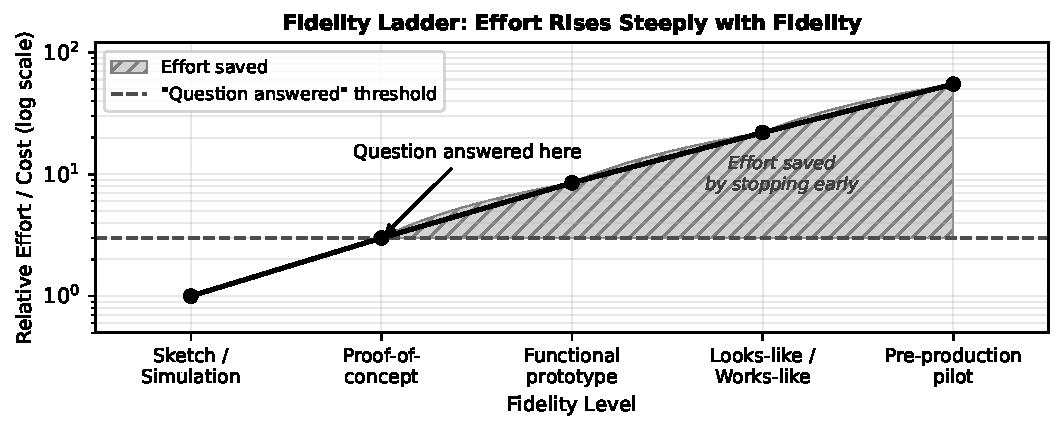
\includegraphics[width=0.85\textwidth]{images/fig_02_fidelity_ladder.pdf}
  \caption{Relative effort rises steeply with fidelity level. A proof-of-concept
           (Level~2) answers many questions at a fraction of the cost of a
           looks-like/works-like prototype (Level~4).}
  \label{fig:ch2-fidelity-ladder}
\end{figure}

\subsection{The Effort--Fidelity Model}
\label{sec:ch2-effort-model}

Let $f \in \{1, 2, 3, 4, 5\}$ be the fidelity level, where $f=1$ is a
hand sketch or simulation and $f=5$ is a pre-production prototype built with
production-intent processes.
Define \textbf{relative effort}\index{effort!relative} $E(f)$ as:

\begin{equation}
  \label{eq:ch2-effort}
  E(f) = E_0 \cdot k^{\,f}, \qquad k > 1
\end{equation}

where $E_0$ is a baseline effort constant and $k$ is the per-level effort
multiplier.
The model captures the empirical observation that each fidelity step requires
roughly $k$ times the total effort of the step below it, because higher
fidelity demands tighter tolerances, more sophisticated tooling, more thorough
testing, and more documentation.

\subsubsection*{Worked Example: Effort Table}

Set $E_0 = 1$ and $k = 2.5$ as representative values.
Table~\ref{tab:ch2-effort} shows the resulting effort at each level.

\begin{table}[htbp]
  \centering
  \caption{Relative effort $E(f) = 2.5^{\,f}$ for fidelity levels 1 through~5.}
  \label{tab:ch2-effort}
  \begin{tabular}{cll}
    \hline
    \textbf{Level} $f$ & \textbf{Type} & \textbf{Relative Effort} $E(f)$ \\
    \hline
    1 & Sketch / simulation      & $2.5^1 = 2.5$ \\
    2 & Proof-of-concept         & $2.5^2 = 6.25$ \\
    3 & Functional prototype     & $2.5^3 = 15.6$ \\
    4 & Looks-like/works-like    & $2.5^4 = 39.1$ \\
    5 & Pre-production           & $2.5^5 = 97.7$ \\
    \hline
  \end{tabular}
\end{table}

The ratio of effort at $f=5$ relative to $f=2$ is:
\begin{equation}
  \label{eq:ch2-effort-ratio}
  \frac{E(5)}{E(2)} = \frac{k^5}{k^2} = k^3 = 2.5^3 = 15.6
\end{equation}

If your question is answered at $f=2$, building to $f=5$ multiplies your
effort by $15.6\times$.
Equivalently, $\frac{E(5) - E(2)}{E(5)} \approx 93\,\%$ of the total
$f=5$ effort is \emph{spent after the question is already answered}.
That is the waste the fidelity discipline prevents.

\subsection{Running Example: Choosing Fidelity for the Sorter}
\label{sec:ch2-sorter-fidelity}

Return to the central question for the connected IoT robotic sorting
subsystem:

\begin{quote}
  ``Can a sub-\$500~CAD BOM sorter module achieve $\geq$95\,\% sort accuracy
  at 6~items/min with reliable MQTT connectivity over standard Wi-Fi?''
\end{quote}

The team is deciding between two prototype options:

\begin{description}
  \item[Option~A --- Looks-like/works-like ($f=4$):]
    Custom PCB with production layout, injection-moulded housing mock-up,
    full production firmware with over-the-air update support.
    Estimated build time: 14~weeks.

  \item[Option~B --- Proof-of-concept ($f=2$):]
    Breadboard electronics, 3D-printed mounting bracket, firmware with sort
    accuracy event logging, Wi-Fi MQTT connectivity test.
    Estimated build time: 3~weeks.
\end{description}

Applying the effort model with $k=2.5$:
\begin{equation}
  \label{eq:ch2-sorter-ratio}
  \frac{E(4)}{E(2)} = k^{4-2} = 2.5^2 = 6.25
\end{equation}

Option~A requires $6.25\times$ the effort of Option~B.
Now ask: does the central question require $f=4$?
The question asks about sort accuracy, throughput rate, BOM cost, and MQTT
connectivity.
None of those require an injection-moulded housing or a production PCB.
A breadboard can deliver accurate sensor readings; a 3D-printed bracket can
hold the actuator at the required geometry; a Wi-Fi module on a breadboard
can carry MQTT traffic.

The decision is Option~B.
If Option~B answers ``yes,'' the team proceeds to Milestone~2 with the
validated architecture, and Option~A becomes the correct investment at that
stage.
If Option~B answers ``no'' --- the sort accuracy is 78\,\% at 6~items/min,
or the MQTT latency is unacceptable on a congested network --- the team has
lost 3~weeks, not 14.
The cost of a wrong hypothesis is bounded by the fidelity choice.

\paragraph{Common Pitfalls.}
\begin{itemize}
  \item \textbf{``Prototype = mini-product.''}\index{pitfall!prototype as mini-product}
    Building all product features when only one needs to be proved is the
    most common and most expensive prototyping error.
    Injection moulding, CE certification, and production firmware are
    irrelevant at Stage~4 if the question is about sort accuracy.
    Every feature you build beyond what the question requires is pure waste
    until the question is answered.

  \item \textbf{``Higher fidelity is always better.''}\index{pitfall!over-fidelity}
    Fidelity costs effort exponentially, as shown in
    Table~\ref{tab:ch2-effort}.
    A higher-fidelity prototype that cannot yet answer the question delivers
    zero additional information --- it only consumes schedule and budget.
    Match fidelity to the question; resist the instinct to impress.
\end{itemize}

%%%%%%%%%%%%%%%%%%%%%%%%%%%%%%%%%%%%%%%%%%%%%%%%%%%%%%%%%%%%%%%%%%%%%%%%%%%
\section*{End-of-Chapter Artifact}
\label{sec:ch2-artifact}
%%%%%%%%%%%%%%%%%%%%%%%%%%%%%%%%%%%%%%%%%%%%%%%%%%%%%%%%%%%%%%%%%%%%%%%%%%%

\addcontentsline{toc}{section}{End-of-Chapter Artifact}

The deliverable for this chapter is a single written paragraph, submitted
to your portfolio, stating: (1) the central question your Milestone~1
prototype will answer, (2) the fidelity level you have chosen, and (3) a
justification for that choice in terms of the question, the risk it retires,
and the effort saved relative to the next higher fidelity level.

\bigskip
\noindent\textbf{Running-Example Statement (model your own on this):}

\begin{quote}
The Milestone~1 prototype for the IoT robotic sorting subsystem will answer
the following central question: \emph{``Can a sub-\$500~CAD BOM sorter
module achieve $\geq$95\,\% sort accuracy at 6~items/min with reliable MQTT
connectivity over standard Wi-Fi?''}
The chosen fidelity is Level~2 (proof-of-concept), implemented as breadboard
electronics, a 3D-printed mechanical mounting bracket, and firmware with
sort-event data logging and Wi-Fi MQTT connectivity.
This fidelity is sufficient because the question is about sensor accuracy,
actuator throughput, and network protocol performance --- none of which
require a production PCB layout or an enclosure.
Advancing to Level~4 at this stage would multiply effort by $6.25\times$
(Equation~\ref{eq:ch2-sorter-ratio}) before the feasibility of the core
mechanism is established.
If the Level~2 prototype answers ``yes,'' Level~4 is the justified next
investment; if ``no,'' the team reframes the architecture having lost
3~weeks rather than~14.
\end{quote}

This statement feeds directly into the specification document you will
develop in Chapter~4.
Keep it in your portfolio; you will reference and refine it at each
subsequent milestone.

%%%%%%%%%%%%%%%%%%%%%%%%%%%%%%%%%%%%%%%%%%%%%%%%%%%%%%%%%%%%%%%%%%%%%%%%%%%
\section*{Chapter Summary}
\label{sec:ch2-summary}
%%%%%%%%%%%%%%%%%%%%%%%%%%%%%%%%%%%%%%%%%%%%%%%%%%%%%%%%%%%%%%%%%%%%%%%%%%%

\addcontentsline{toc}{section}{Chapter Summary}

A prototype is the minimum sufficient artifact that answers a specific
technical or business question and retires a corresponding risk.
The Prototype Development Cycle organises that work into seven stages:
Stage~1 (Specification \& Risk) establishes what must be true and what is
assumed; Stage~2 (Scoping \& Planning) sets the question, the fidelity,
and the success criterion; Stage~3 (Architecture) partitions the system
into subsystems with defined interfaces; Stage~4 (Subsystem Design) produces
the design artefacts; Stage~5 (Build \& Integration) realises and assembles
those designs; Stage~6 (Validate \& Measure) answers the question against
pre-defined criteria; and Stage~7 (Compile \& Economics) closes the milestone
with evidence and a go/no-go recommendation.

Stages~4 through~6 form a controlled iteration loop.
Each pass tests one hypothesis, changes one variable, and exits on a
measured criterion --- not on a deadline and not by accumulated intuition.

Fidelity is not a virtue.
It is a variable you set to the minimum level that makes the central
question answerable.
The effort--fidelity relationship is exponential ($E(f) = E_0 \cdot k^f$),
so every unnecessary fidelity level you add multiplies your cost by $k$
before you have an answer.
For the sorter running example, choosing Level~2 over Level~4 saves
$6.25\times$ the effort on a question whose answer is not yet known.

\bigskip
\noindent\textbf{Transition to Chapter~3.}
Chapter~3 examines the boundary between prototype and product in detail.
You will learn to distinguish which subsystems require prototyping and which
can be specified directly from validated prior art, and how to apply
\emph{selective prototyping} to allocate your build budget to the risks that
matter.
